\chapter{結論}
\label{conclusion}

本章では,本研究のまとめと今後の課題を示す.

\section{本研究のまとめ}

実験が全て完了したのちにまとめる

\section{本研究の課題}

本研究では, 自動車に限りモビリティーの利用者の満足度を高める経路制御を行う機械的な手法に取り組んだ.
しかし,

\subsection{想定環境の貧弱さ}

本研究では, 事前に選び出した幹線道路とその周辺にある主たる施設のみの仮想環境をソフトウェアで再現した. 
しかし, 実際には交通機関は自動車意外にもあり鉄道やバスなどの大量輸送型の交通機関

\subsection{学習器の連携}

本研究では深層強化学習が利用者の満足度を高めるという視点で制御を行えるか実験を行った.
ただ, 実際に本研究の手法を適用する場合, 



\begin{figure}[H]
    \centering
    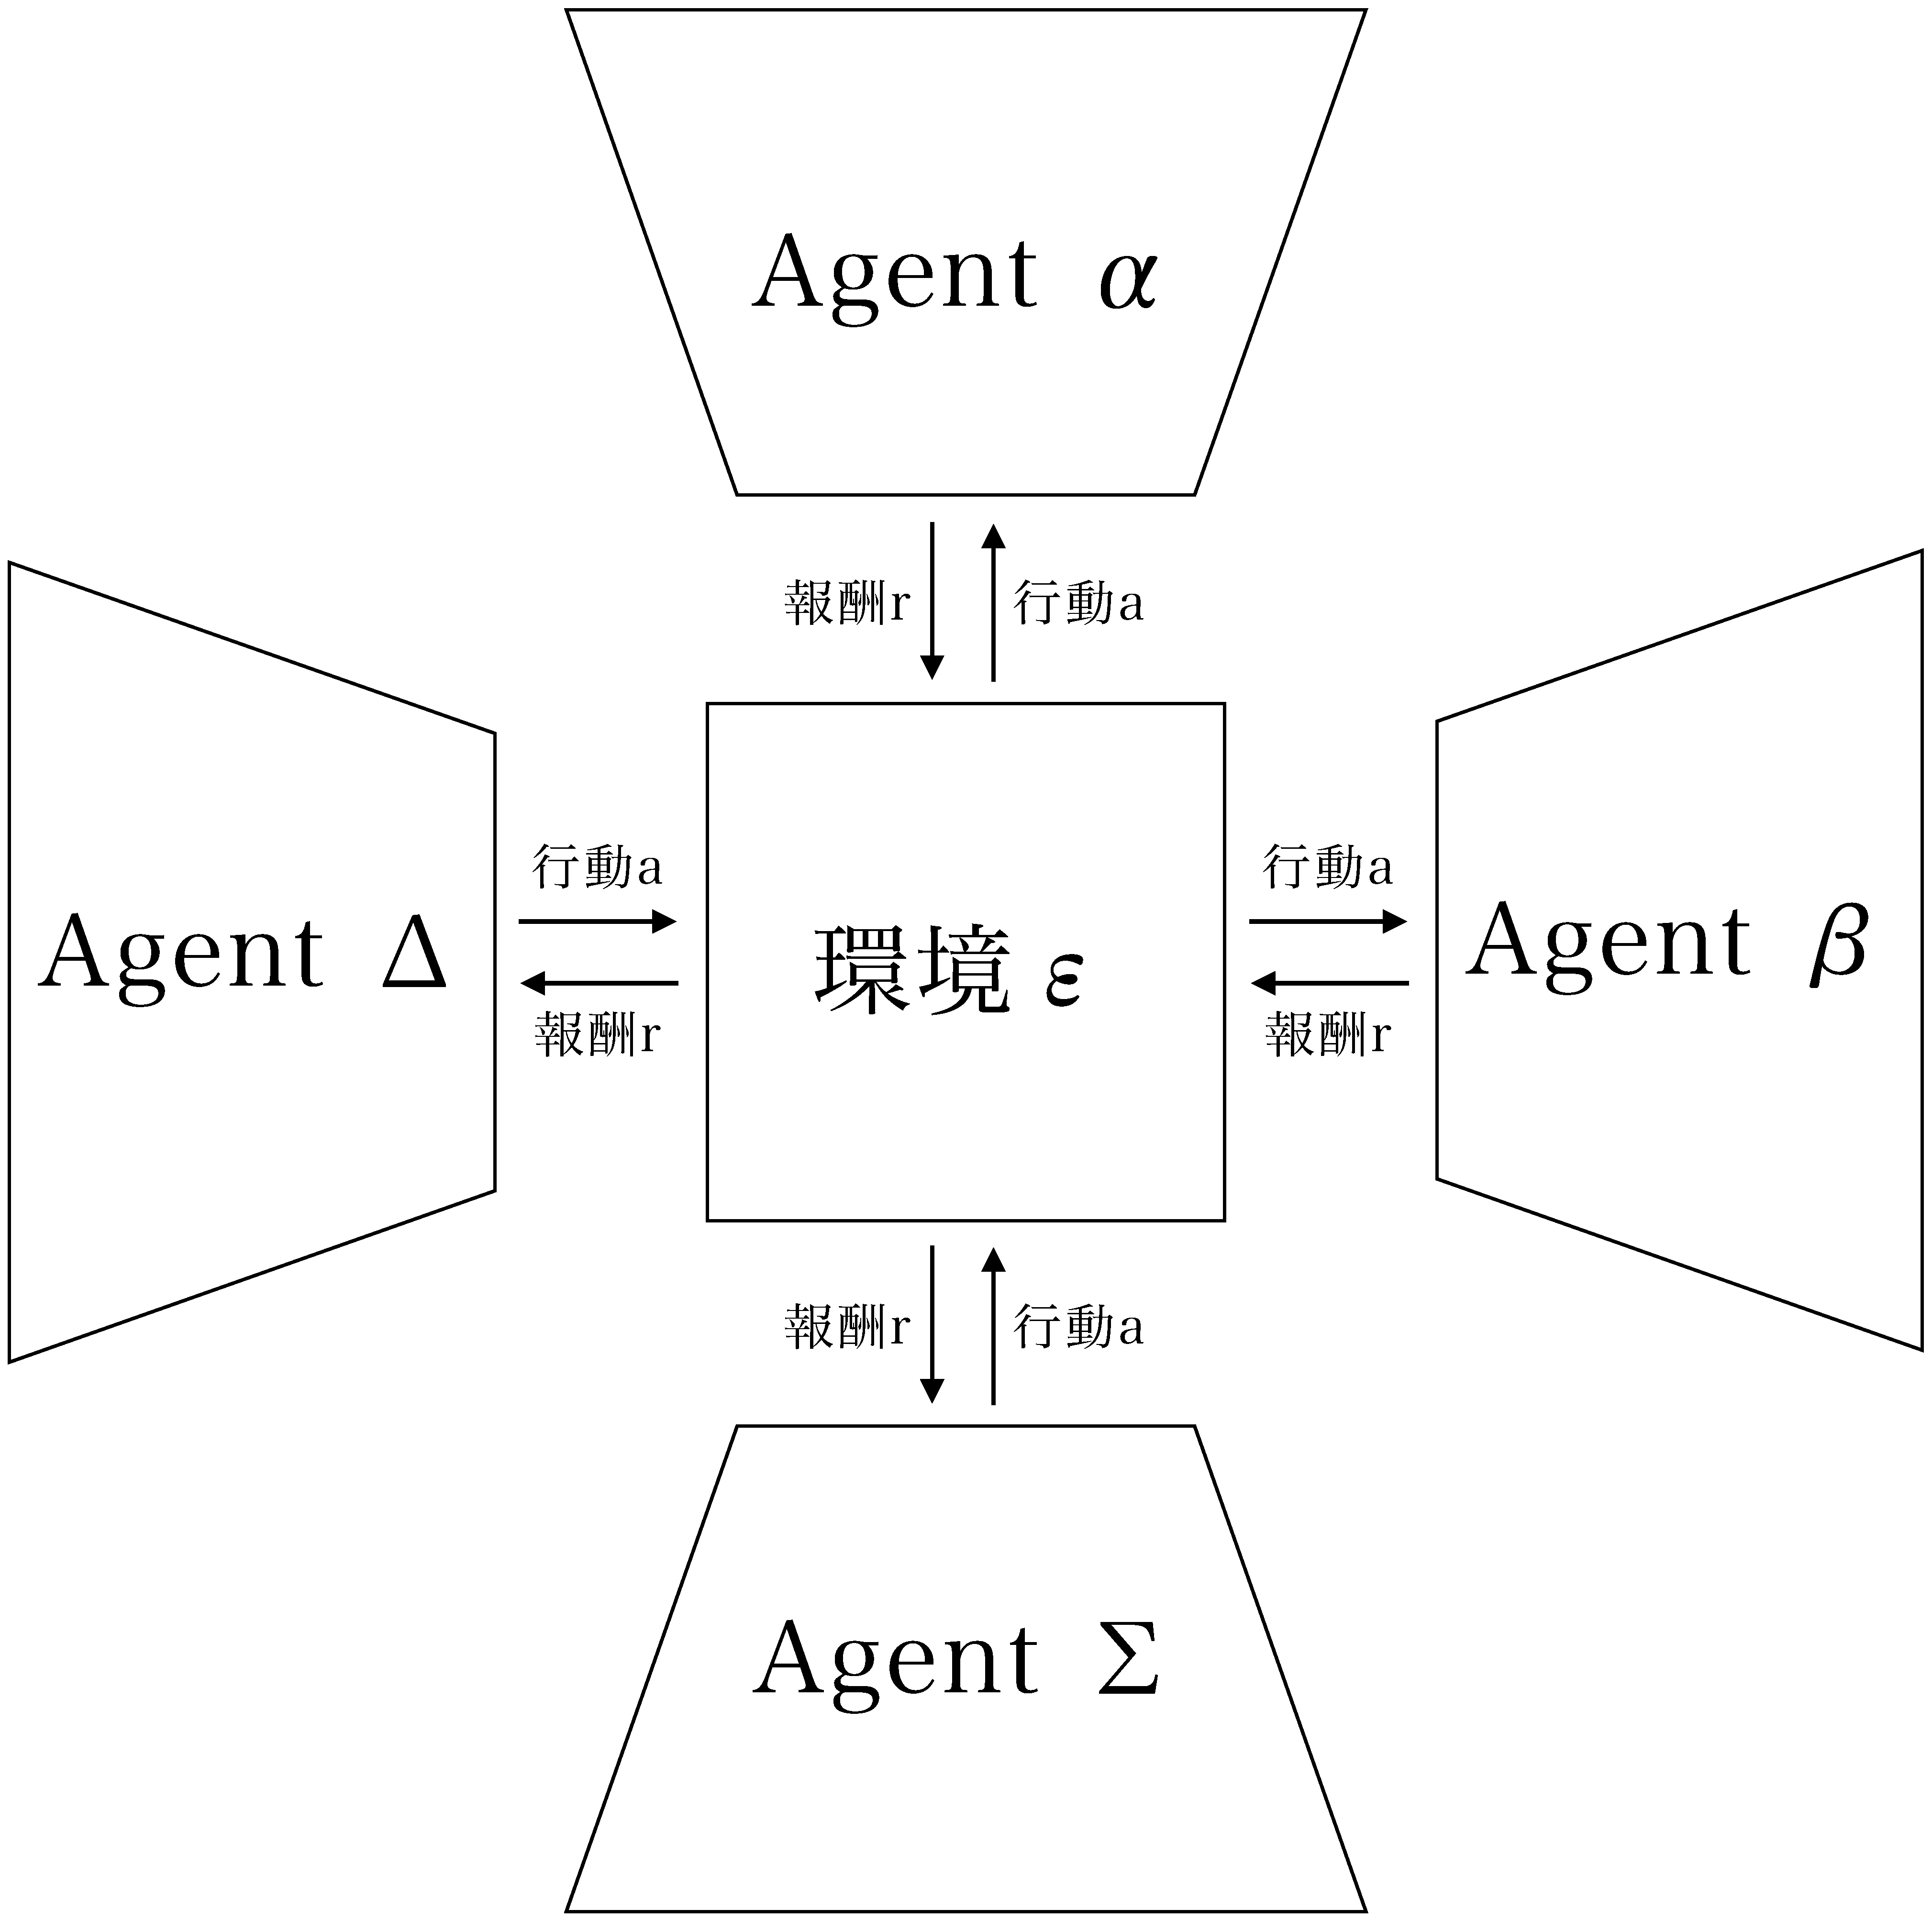
\includegraphics[clip,width = 12.0cm]{assets/multiagent_shared_env.eps}
    \caption{複数エージェントで環境を共有する概念図}  \label{sample}
\end{figure}

%%% Local Variables:
%%% mode: japanese-latex
%%% TeX-master: "../thesis"
%%% End:
